\documentclass[a4j,11pt]{ltjsarticle}    % 文章クラスとオプション設定
%%%%%%%%%% スタイル %%%%%%%%%%%%%%%%%%%%%%%%%%%%%%%%%%%%%%%%%%%%%%%%%%%%%%%%%%%%%%%%%%%%%%%%%%%%%%

\usepackage{comment}    % 複数行コメント

% 余白の調整
\usepackage[top=30truemm,bottom=30truemm,left=20truemm,right=20truemm]{geometry}

% 数式関連
\usepackage{amsmath,amssymb,nccmath,siunitx}    % 数式
\usepackage{bm}         % ベクトルの太文字

% 画像関連
\usepackage{graphicx} % 画像

\usepackage{here}% figureの位置調整
% 表設定
\usepackage{multirow}   % 表の行の結合
\usepackage{longtable}  % ページをまたぐ長い表

\usepackage{url}

%%%%%%%%%% 本文 %%%%%%%%%%%%%%%%%%%%%%%%%%%%%%%%%%%%%%%%%%%%%%%%%%%%%%%%%%%%%%%%%%%%%%%%%%%%%%%%%

\begin{document}

% !TEX root = main.tex

%%%%%%%%%%%%%%%%%%%%%%%%%%%%%%%%%%%%%%%%%%%%%%%%%%%%%%%%%%%%%%%%%%%%%%%%%%%%%%%%%%%%%%%%%%%%%%%%

\title{静電場の解析(前半)}
\date{}
\author{}
\maketitle


%%%%%%%%%%%%%%%%%%%%%%%%%%%%%%%%%%%%%%%%%%%%%%%%%%%%%%%%%%%%%%%%%%%%%%%%%%%%%%%%%%%%%%%%%%%%%%%%
% !TEX root = main.tex

%%%%%%%%%%%%%%%%%%%%%%%%%%%%%%%%%%%%%%%%%%%%%%%%%%%%%%%%%%%%%%%%%%%%%%%%%%%%%%%%%%%%%%%%%%%%%%%%
\section{目的}
%%%%%%%%%%%%%%%%%%%%%%%%%%%%%%%%%%%%%%%%%%%%%%%%%%%%%%%%%%%%%%%%%%%%%%%%%%%%%%%%%%%%%%%%%%%%%%%%

等角写像法の原理を理解し,その技法から得られる等電位面と電気力線の関係を視覚的
に描く.また数値計算により,種々の形状をした電極電位が作り出す等電位面を求め,静電
場$\vec{E}$の様子を理解する.更には,実験で用いた平行平板電極のセットアップに即した等電位
面を数値計算ソフトを用いて可視化する.最後に,実験で得られた電位$V$の空間分布を解
析解比較し,電極エッジ効果を理解する.

% !TEX root = main.tex

%%%%%%%%%%%%%%%%%%%%%%%%%%%%%%%%%%%%%%%%%%%%%%%%%%%%%%%%%%%%%%%%%%%%%%%%%%%%%%%%%%%%%%%%%%%%%%%%
\section{原理}
%%%%%%%%%%%%%%%%%%%%%%%%%%%%%%%%%%%%%%%%%%%%%%%%%%%%%%%%%%%%%%%%%%%%%%%%%%%%%%%%%%%%%%%%%%%%%%%%

\subsection{対角写像法}
電極に与えられた電位$V_0$が作る$V$の空間分布$V(x,y,z)$を求めるには,
ラプラス方程式
$$
\nabla^2 V=\frac{\partial^2 V}{\partial x^2}+\frac{\partial^2 V}{\partial y^2}+\frac{\partial^2 V}{\partial z^2}=0
$$

を2つの境界条件

\begin{itemize}
    \item 導体の電位は一定である.
    \item 誘電体の教会では,電束密度$\vec{D}$の法線方向の成分と$\vec{E}$の接線方向の成分が連続となる.
\end{itemize}

の下で解けば良い.この式は,$V$が2次元でかつ対称性が良い場合,
等角写像を応用することで綺麗に解くことができる.

等角写像とは,ある2つの複素変数$z= (x + iy)とw = (u + iv)$が正則な関数$f$
によって$w =f(z)$と結び付けられているとき,$z$の値を変化させて$z$平面上である
図形を描くと,それぞれの$z$の値に対応する$w$もまた$w$平面上である図形を描く.
このとき,$f(z)$が解析関数である限り,$z$平面上での3点が作る角度
$\angle z_1z_2z_3$と,$w$平面上の対応する3点が作る角度$\angle w_1w_2w_3$
が必ず等しくなる.このような写像を等角写像という.

また,平行平板電極が$x$軸と平行に$y = \pm d$の位置に置かれ,$y = d$の電極に
$V_0$,$y = -d$の電極に$-V_0$の電圧を印加した場合,$V(x,y)$の等電位線は以下の式で
表される軌跡となる.

$$
\begin{aligned}
&x=d\left\{t+\frac{1}{\pi} e^{\pi t} \cos \left(\frac{\pi V}{V_0}\right)\right\} \\
&y=d\left\{\frac{V}{V_0}+\frac{1}{\pi} e^{\pi t} \sin \left(\frac{\pi V}{V_0}\right)\right\}
\end{aligned}
$$

\subsection{数値計算}

数値計算では,数理モデル化によって表された微分方程式を離散化し,
それらによって得られた代数方程式をコンピュータを用いて解析する.

本実験では,Mesh及びEStatというソフトウェアを用いて計算機実験を行い,Meshでは,
有限要素法解析に必要な三角メッシュを生成し,EStatによりポテンシャルの計算を行う.

有限要素法とは,領域を多数の部分領域に分割し,その領域内において単純な関数の重ね
合わせによって未知量を近似する手法である.

% !TEX root = main.tex

%%%%%%%%%%%%%%%%%%%%%%%%%%%%%%%%%%%%%%%%%%%%%%%%%%%%%%%%%%%%%%%%%%%%%%%%%%%%%%%%%%%%%%%%%%%%%%%%
\section{実験}
%%%%%%%%%%%%%%%%%%%%%%%%%%%%%%%%%%%%%%%%%%%%%%%%%%%%%%%%%%%%%%%%%%%%%%%%%%%%%%%%%%%%%%%%%%%%%%%%

\subsection{シミュレーション手順}
\begin{enumerate}
    \item Meshを用いて実験課題にあった領域を作成し,メッシュを作成する.
    \item Estateを用いて,実験課題にあった領域要素(電位,誘電率)を指定し,
    ポテンシャルの計算を行う.その後,解析結果を表示する.本実験では,比誘電率
    を以下のように定める.\\
    水:$80.4(20\si{\celsius})$\quad 空気:$1.00$\quad ガラス:$7.65$\\
    また,印加電圧は$10\,[\si{\volt}]$とする.
\end{enumerate}

\subsection{先週の実験を模擬する}
ソフトフェアを用いて,第一週目の実験セットアップとパラメータの時の等電位面を計
算し,$(x,y)$平面における等電位線を描く.

\subsection{境界の役割を学ぶ}
ソフトウェアを用いて,境界が無限遠とした場合の等電位面を計算する.なお,この計算
においては,電極の厚み$t$と間隔$d$は自由に設定してよい.

\subsection{真空中での電位分布}
ソフトウェアを用いて,媒質が真空の場合の等電位面を計算する.

\subsection{電極形状の影響}
ソフトウェアを用いて,平行平板電極の形状を曲面板とした場合の等電位面を計算する.

% !TEX root = main.tex

%%%%%%%%%%%%%%%%%%%%%%%%%%%%%%%%%%%%%%%%%%%%%%%%%%%%%%%%%%%%%%%%%%%%%%%%%%%%%%%%%%%%%%%%%%%%%%%%
\section{結果}
%%%%%%%%%%%%%%%%%%%%%%%%%%%%%%%%%%%%%%%%%%%%%%%%%%%%%%%%%%%%%%%%%%%%%%%%%%%%%%%%%%%%%%%%%%%%%%%%

\subsection{実験課題1}
シミュレーション結果を以下の図1に示す.$x$座標が正の電極板に$10\,[\si{\volt}]$
の印加電圧がかかっており,$x$座標が負の電極板はGNDに接続しているとする.
\begin{figure}[H]
    \begin{center}
        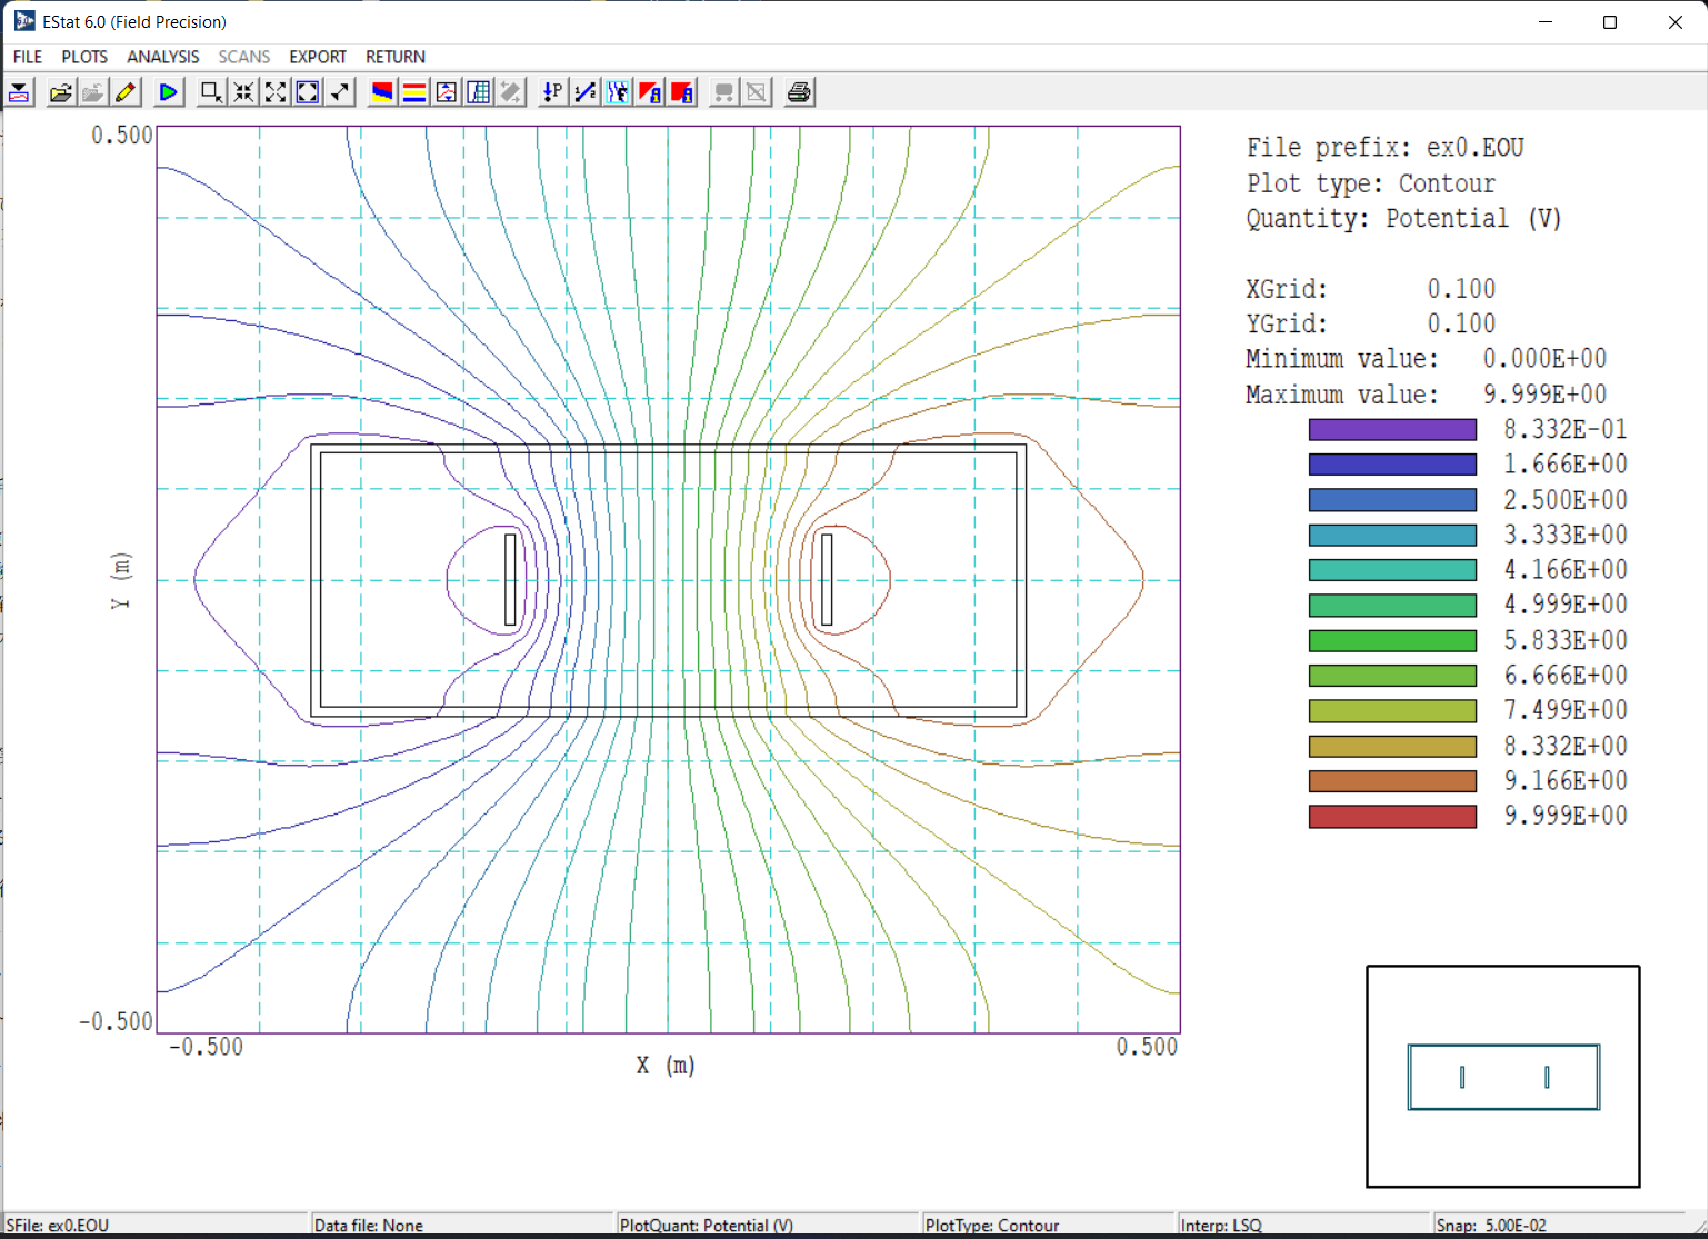
\includegraphics[scale=0.5]{figure1.pdf}
        \caption{第1週目の実験時のセットアップにおける等電位面}
    \end{center}
\end{figure}
\newpage

\subsection{実験課題2}
シミュレーション結果を以下の図2に示す.$x$座標が正の電極板に$10\,[\si{\volt}]$
の印加電圧がかかっており,$x$座標が負の電極板はGNDに接続しているとする.
\begin{figure}[H]
    \begin{center}
        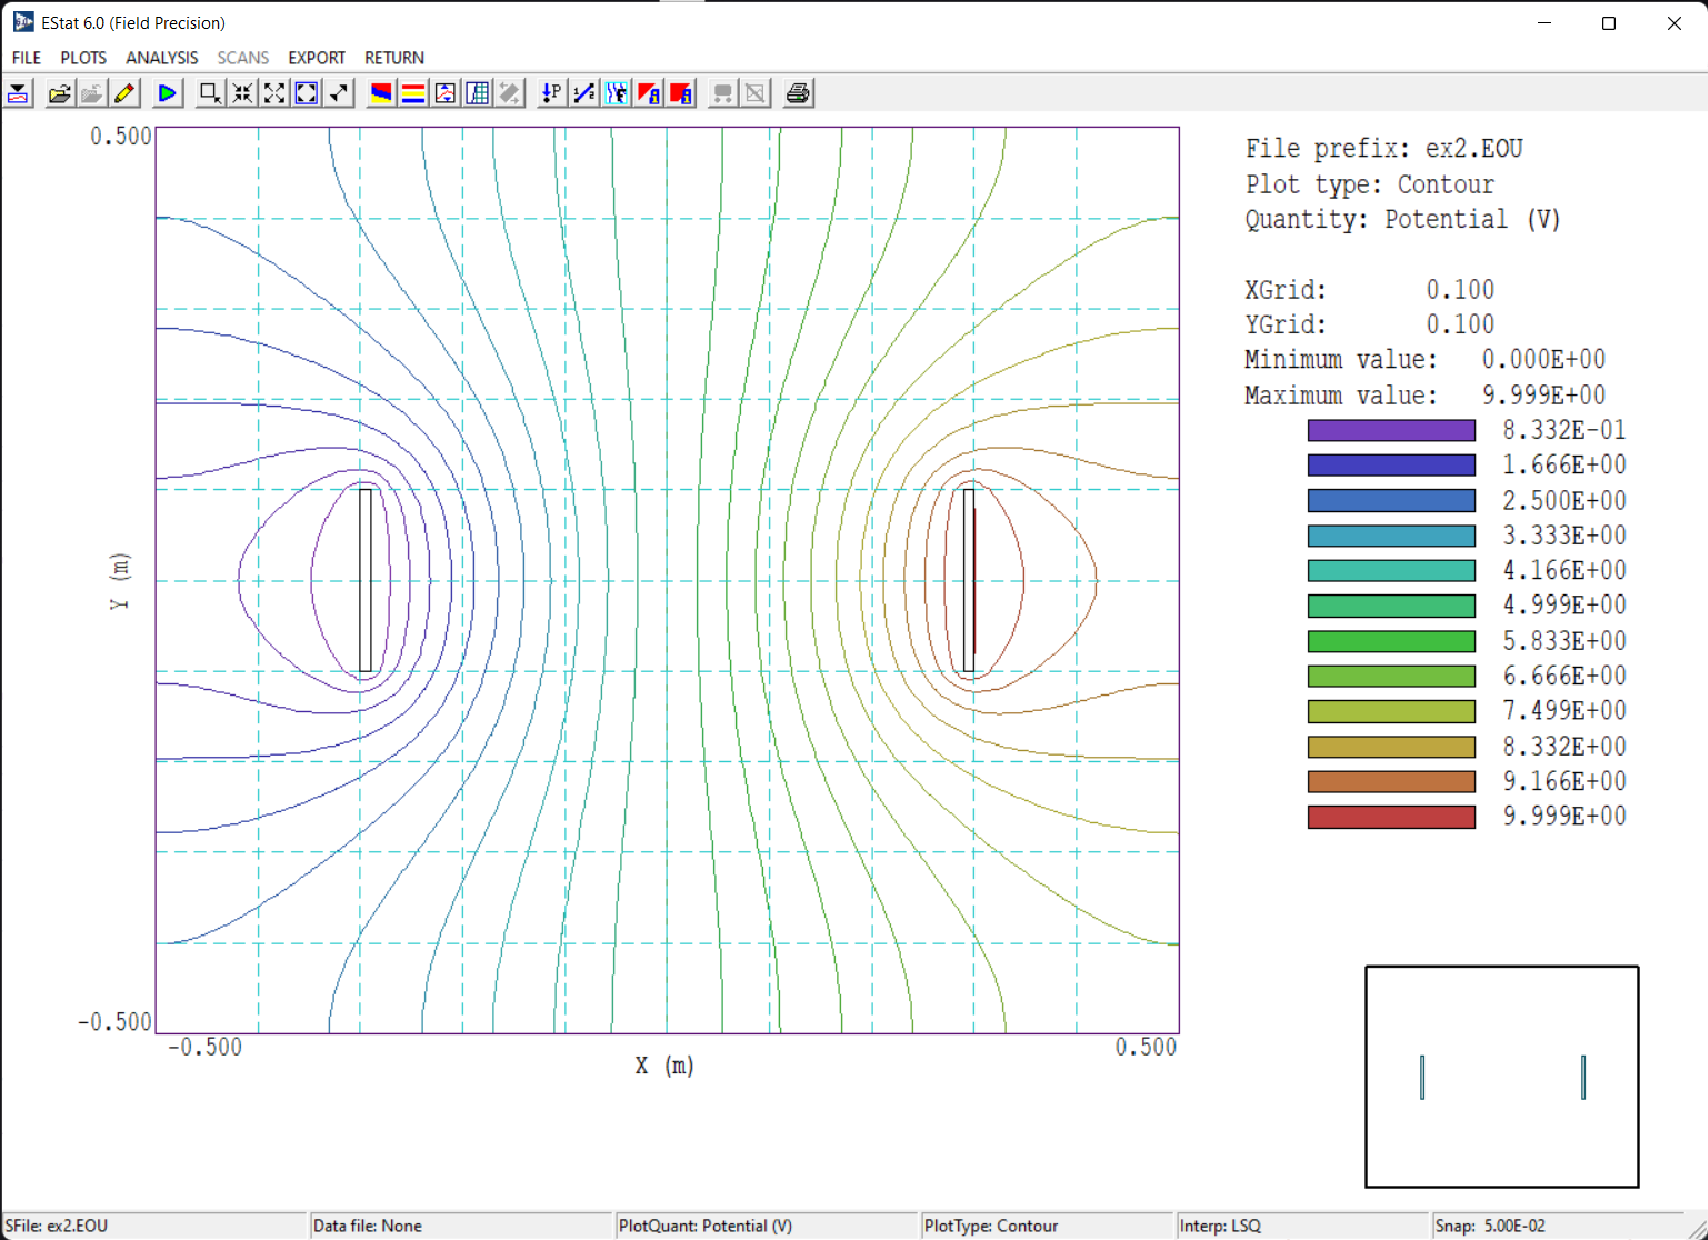
\includegraphics[scale=0.5]{figure2.pdf}
        \caption{境界が無限遠とした場合の等電位面}
    \end{center}
\end{figure}
\newpage

\subsection{実験課題3}
シミュレーション結果を以下の図3に示す.$x$座標が正の電極板に$10\,[\si{\volt}]$
の印加電圧がかかっており,$x$座標が負の電極板はGNDに接続しているとする.
\begin{figure}[H]
    \begin{center}
        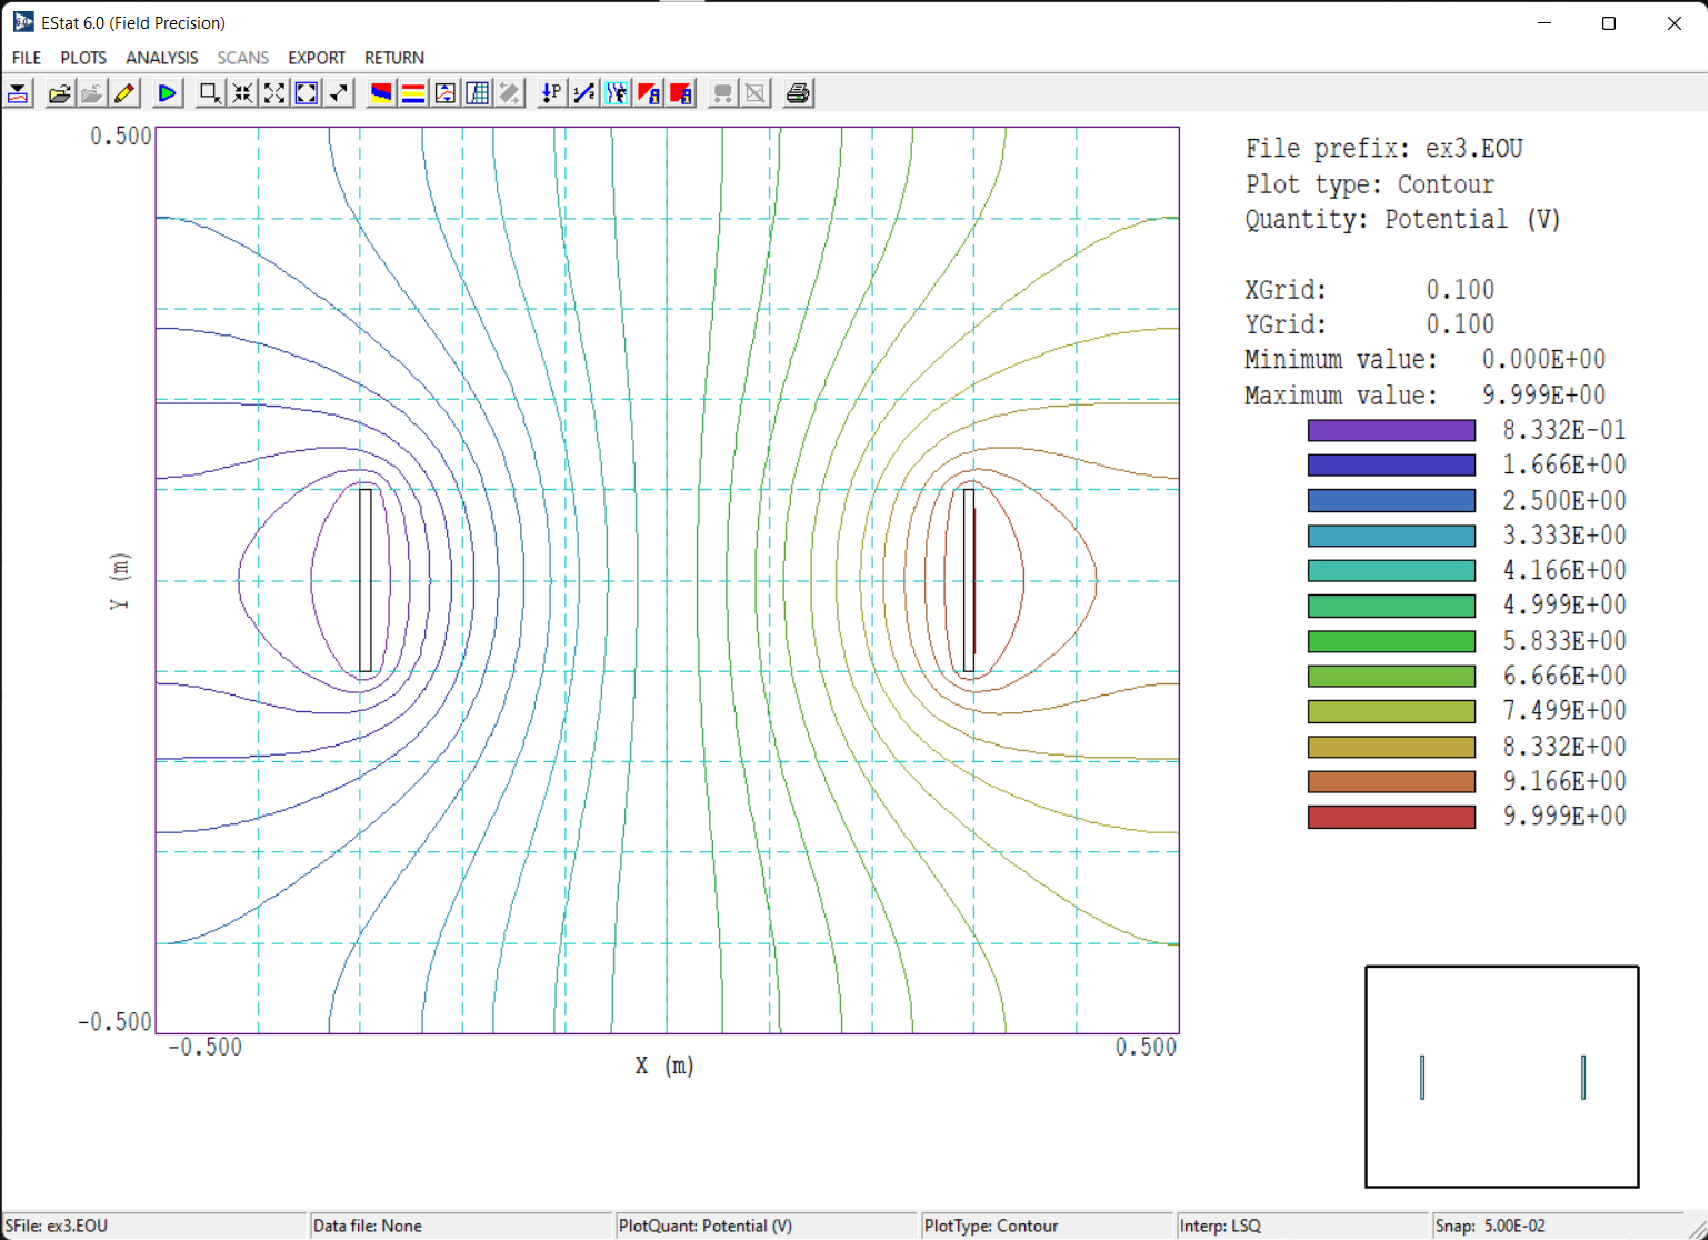
\includegraphics[scale=0.5]{figure3.pdf}
        \caption{媒質が真空の場合の等電位面}
    \end{center}
\end{figure}
\newpage

\subsection{実験課題4}
シミュレーション結果を以下の図4に示す.$x$座標が正の電極板に$10\,[\si{\volt}]$
の印加電圧がかかっており,$x$座標が負の電極板はGNDに接続しているとする.
\begin{figure}[H]
    \begin{center}
        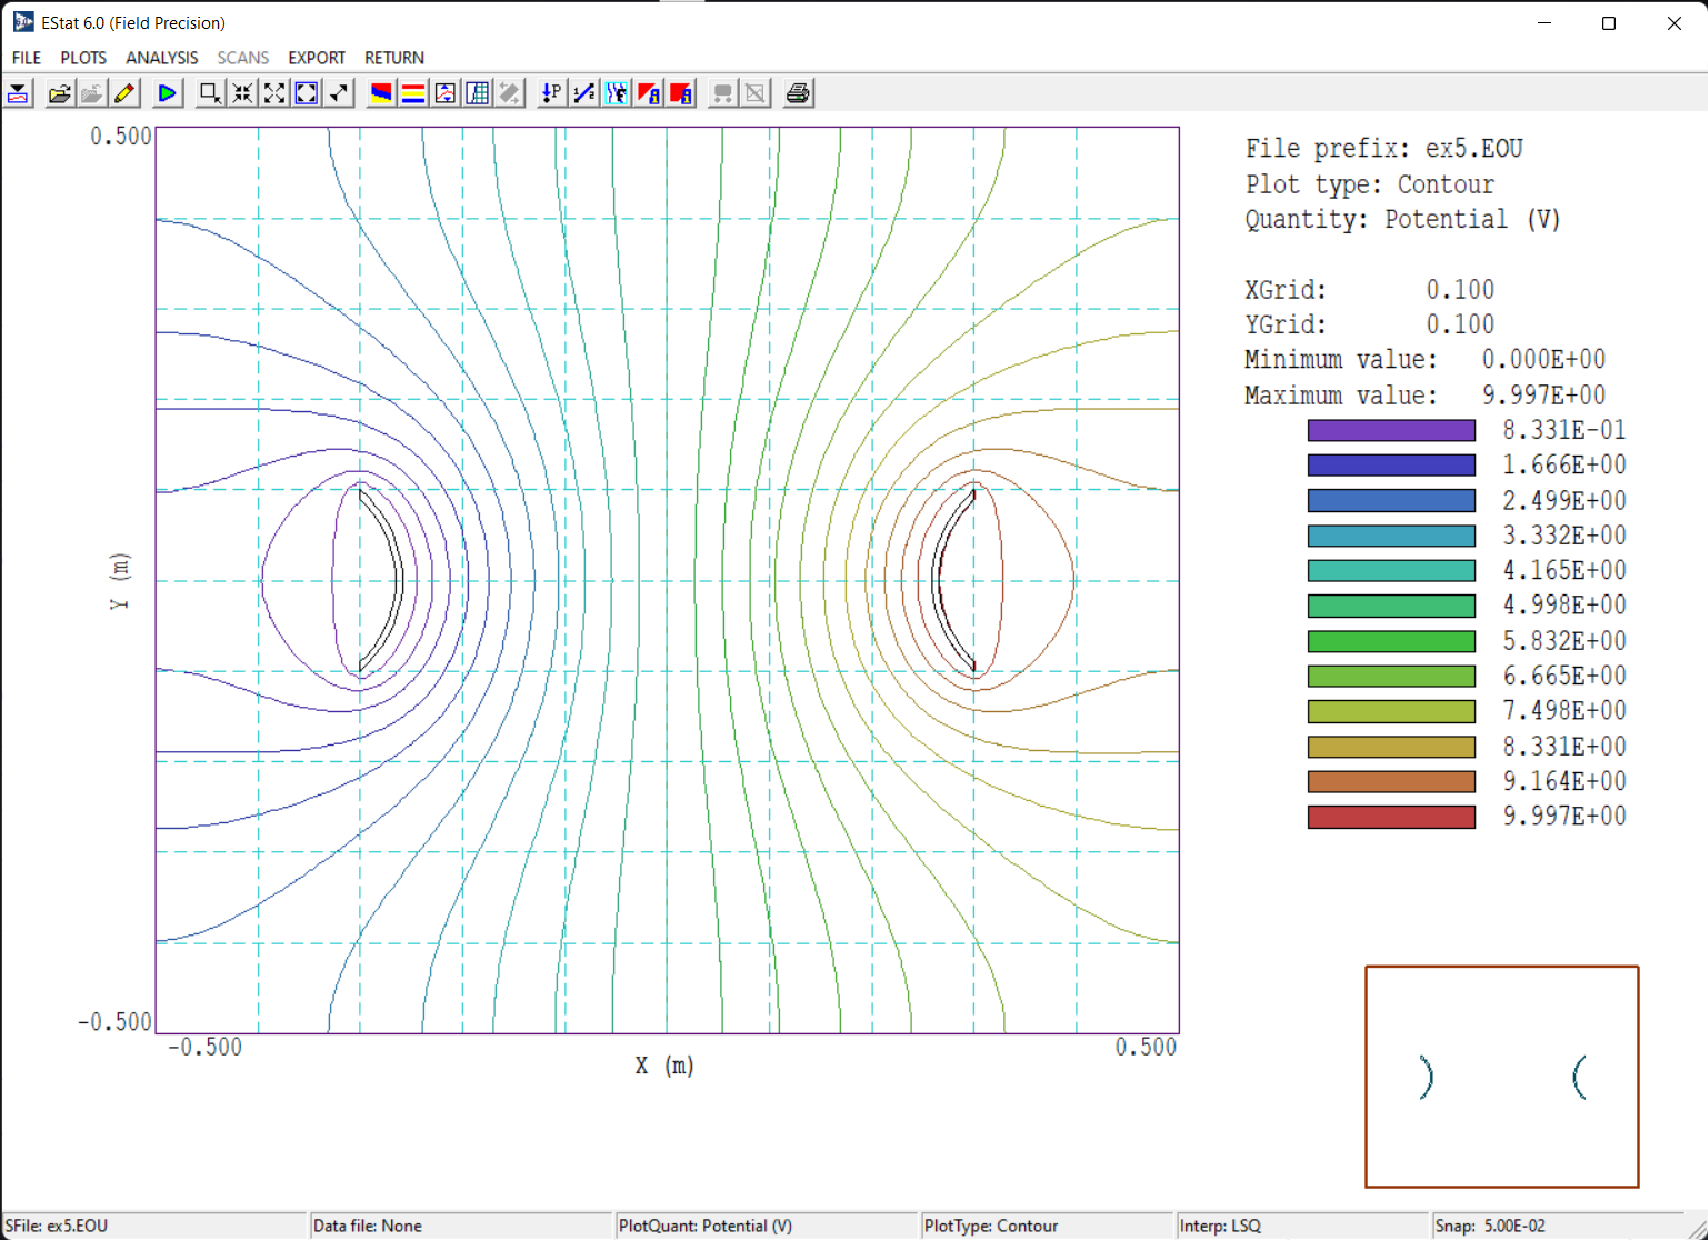
\includegraphics[scale=0.5]{figure4.pdf}
        \caption{電極板が曲面板の場合の等電位面}
    \end{center}
\end{figure}
\newpage
% !TEX root = main.tex

%%%%%%%%%%%%%%%%%%%%%%%%%%%%%%%%%%%%%%%%%%%%%%%%%%%%%%%%%%%%%%%%%%%%%%%%%%%%%%%%%%%%%%%%%%%%%%%%
\section{データ解析と考察}
%%%%%%%%%%%%%%%%%%%%%%%%%%%%%%%%%%%%%%%%%%%%%%%%%%%%%%%%%%%%%%%%%%%%%%%%%%%%%%%%%%%%%%%%%%%%%%%%

\begin{enumerate}
    \item 計算機実験の結果を第一週で得た電位𝑉の空間分布実験結果の上に上書きせよ.
    そして,それらを比較して,一致点と相違点を全て列挙せよ.
    \begin{description}
        \item[] 計算機実験の結果を第1週で得た電位$V$の空間分布実験結果の上に
        上書きしたものを図5に示す.
    \end{description}
    
    \begin{itemize}
        \item 一致点
        \begin{description}
            \item[] $y$座標が小さくなるほどが原点に引っ張られるような等電位線となっており,
            $x$座標が正において「く」の字型,$x$座標が負において,逆「く」の字型になっている.
        \end{description}

        \item 相違点
        \begin{description}
            \item[] 
        \end{description}
    \end{itemize}

    \item 設問(1)における相違点が現れてきた理由を説明せよ.
    \begin{description}
        \item[] 
    \end{description}
\end{enumerate}
% !TEX root = main.tex

%%%%%%%%%%%%%%%%%%%%%%%%%%%%%%%%%%%%%%%%%%%%%%%%%%%%%%%%%%%%%%%%%%%%%%%%%%%%%%%%%%%%%%%%%%%%%%%%
\section{宿題}
%%%%%%%%%%%%%%%%%%%%%%%%%%%%%%%%%%%%%%%%%%%%%%%%%%%%%%%%%%%%%%%%%%%%%%%%%%%%%%%%%%%%%%%%%%%%%%%%

\begin{enumerate}
    \item 第1週目で行った実験時のセットアップ値を(19)式
    に代入することで,貴方の実験グループの解析解を示せ.
    \begin{description}
        \item[] 第1週目に行った実験のパラメータは,
        $d = 150\,[\si{mm}],V_0 = 5\,[\si{\volt}]$であるので,解析解は次のようになる.
        $$
        x=150\left\{t+\frac{1}{\pi} e^{\pi t} \cos \left(\frac{\pi V}{5}\right)\right\}[\mathrm{mm}], y=150\left\{\frac{V}{5}+\frac{1}{\pi} e^{\pi t} \sin \left(\frac{\pi V}{5}\right)\right\}[\mathrm{mm}]
        $$
    \end{description}

    \item 実験課題3より分かるように,媒質が真空でも等電位面は存在しているが,
    真空中では実験で用いたプローブから信号出力を得ることはできない.
    この理由を説明せよ.
    \begin{description}
        \item[] 水の比誘電率が$80.4(20\si{\celsius})$であるのに対し,
        真空の比誘電率は$8.8541\times 10^{-12}$である.
        そのため媒質が水の場合と比べて,真空中では電場が非常に小さくなり,
        電場によって生じる電流が小さくなる.真空中では媒質中に流れる電流値が
        実験で用いたプローブの電流測定が可能な範囲よりも小さくなるため,
        信号出力を得ることはできないと考えられる.
    \end{description}
\end{enumerate}

%%%%%%%%%% 参考文献 %%%%%%%%%%%%%%%%%%%%%%%%%%%%%%%%%%%%%%%%%%%%%%%%%%%%%%%%%%%%%%%%%%%%%%%%%%%%%%

% !TEX root = main.tex

%%%%%%%%%% 参考文献 %%%%%%%%%%%%%%%%%%%%%%%%%%%%%%%%%%%%%%%%%%%%%%%%%%%
\begin{thebibliography}{99}
    \newcounter{num}
    \setcounter{num}{2}
    \bibitem{電子システム工学基礎実験テキスト}
\end{thebibliography}

\end{document}